%%%%%%%%%%%%%%%%%%%%%%%%%%%%%%%%%%%%%%%%%%%%%%%%%%%%%%%%%%%%%%%%%%%%%%%%
% Plantilla TFG/TFM
% Escuela Politécnica Superior de la Universidad de Alicante
% Realizado por: Jose Manuel Requena Plens
% Contacto: info@jmrplens.com / Telegram:@jmrplens
%%%%%%%%%%%%%%%%%%%%%%%%%%%%%%%%%%%%%%%%%%%%%%%%%%%%%%%%%%%%%%%%%%%%%%%%

\chapter{Metodología}
\label{metodologia}

    - Explicar diagrama de flujo
        - Cada uno de los i apartados (limpieza, etc.) --> especial hincapié a los datos (explicar los datos): 

            - Fuente de datos
            - Columnas
            - Consideraciones de limpieza

            - Analisis y tratamiento de datos -> meter las cuatro cajtas. y meter también análisis

El desarrollo de este proyecto respeta tanto el proceso de desarrollo \textit{Software} como el ciclo de vida de proyectos de \textit{Ciencia de Datos}, por lo que se ha dividido en varias fases acontecidas que definiremos a continuación en base a la planificación mediante un \textit{Diagrama de Gantt}:


\section{Diagrama de flujo}


    \begin{figure}[h]
        \centering
        \includesvg[inkscapelatex=false]{archivos/DataflowImage}
        \caption{Flujo de datos del proceso del proyecto.}
        \label{DataflowImage}
    \end{figure}

\section{Diagrama de Gantt}

    \begin{figure}[h]
        \centering
        \includesvg[inkscapelatex=false]{archivos/GranttImage}
        \caption{Diagrama de Gantt de la planificación del proyecto.}
        \label{GranttImage}
    \end{figure}

\section{Proceso}

    En esta sección describiremos cada uno de los pasos que ha seguido el desarrollo del proyecto, desde la búsqueda inicial de datos hasta la implementación final de los algoritmos:

    \begin{enumerate}

        \item Datos

            El conjunto de datos con el que se ha trabajado en este proyecto describe accidentes de tráfico de la ciudad de Madrid en un periodo concreto, desde el año 2019 hasta el 2022. Este dataset ha sido obtenido desde la fuente del portal de datos abiertos de Madrid \cite{Dataset}, donde es posible encontrar conjuntos de datos de distinta naturaleza relativos a la ciudad de Madrid.

            El número total de registros en este periodo de tiempo es de 60966 instancias, cada una de las cuales consta de 17 características que se describirán en la tabla \ref{DescripcionDatosTabla}:

            \begin{table}[h]
                \centering
                    \begin{tabular}{p{0.35\linewidth} | p{0.6\linewidth}}
                        Atributo&Descripción\\
                        \hline
                        \texttt Número de expediente&Identificador del incidente, si varios registros tienen el mismo un número de expediente se consideran como un mismo incidente y cada registro representa distintas personas involucradas en el incidente (Conductor, Pasajero o Peatón).\\
                        \texttt Fecha&Día mes y año en el que se ha producido el incidente.\\
                        \texttt Hora&Hora y minuto del día.\\
                        \texttt Localización&Nombre de la calle.\\
                        \texttt Número&Número de la calle.\\
                        \texttt Distrito&Nombre del distrito de Madrid.\\
                        \texttt Tipo de accidente&Tipología de accidente (Colisión doble, Colisión múltiple, Alcance, Choque contra obstáculo, Atropello, Vuelco, Caída, Otras causas)\\
                        \texttt Estado meteorológico&Condiciones climatológicas en el momento del incidente (Despejado, Nublado, Lluvia débil, Lluvia intensa, Granizado o Nevando)\\
                        \texttt Tipo de vehículo&\\
                        \texttt Tipo de persona&Persona que ha sido involucrada en el incidente (Conductor, Pasajero o Peatón)\\
                        \texttt Rango de edad&\\
                        \texttt Sexo&Sexo de la persona involucrada (Hombre o Mujer)\\
                        \texttt Lesividad&\\
                        \texttt Coordenada X&Coordenada X del accidente en formato \textit{UTM}\\
                        \texttt Coordenada Y&Coordenada Y del accidente en formato \textit{UTM}\\
                        \texttt Positivo en alcohol&Si la persona implicada ha dado positivo en el control de alcoholemia (S o N)\\
                        \texttt Positivo en drogas&Si la persona implicada ha dado positivo en el control de alcoholemia (S o N)\\ \hline
                    \end{tabular}
                    \caption{Descripción de los datos.}
                    \label{DescripcionDatosTabla}

            \end{table}


            Se pueden consultar los más detalles de las características del dataset descripción del conjunto de datos del portal \textit{Open Data} de Madrid \cite{InfoDatasetMadrid}.\\


            \begin{enumerate}

                \item Limpieza de datos

                    Una vez importados los datos en el proyecto, es requisito hacer una limpieza de éstos (\textit{Data Cleaning}), eligiendo las características que serán utilizadas como variables explicativas en las predicciones atendiendo además a los valores de las instancias, ya que pueden contener valores nulos, valores atípicos (\textit{outliers}) o contener valores erróneos. Esta problemática requiere de estrategias a la hora de tratar estos valores.\\

                    En el caso del dataset de accidentes de tráfico de este proyecto se han escogido las siguientes características como variables explicativas \textit{hora, distrito, tipo accidente, estado meteorológico, tipo vehiculo, tipo persona, rango edad, sexo, positivo alcohol, positivo drogas, vehiculos implicados, coordenada x utm, coordenada y utm}.\\


                    Una vez que se han obtenido los predictores con los que trabajarán los modelos, se han eliminado aquellos registros duplicados y aquellos que tuvieran algún valor nulo en alguno de sus predictores. Por lo tanto, las dimensiones finales del conjunto de datos pasarán a ser 12 variables y 54364 registros con respecto a las 17 columnas y 60966 filas originales.\\



                \item Transformaciones de datos


                    En primer lugar ha sido necesario transformar las columnas \textit{coordenada x utm} y \textit{coordenada y utm} a números enteros para que los modelos los puedan tratar. Inicialmente estos valores estaban establecidos como String, sin seguir un formato de decimales estandarizado, por lo que se ha tenido que crear un proceso que analizase cada casuístca y los tradujese a un formato estandarizado.


                    Las columnas \textit{positiva alcohol} y \textit{positiva drogas} se han unido en una nueva columna debido a la cantidad de valores nulos que existía en la segunda variable, por lo que se crea una nueva columna que hace referencia a la intoxicacion etílica o estupefaciente.

                    Para que una \textit{CNN} pueda entrenarse en base a los datos de entrenamiento estos deben ser numéricos, por lo tanto se requiere de una serie de transformacíones que migren los datos categóricos a valores numéricos con el objetivo de que la \textit{CNN} pueda interpretar los datos de entrada como una imagen.

                    Como el objetivo del proyecto es detectar la gravedad del accidente y éste se interpreta según la lesividad de cada una de las personas implicadas, se han transformado los valores de la característica \textit{lesividad} de acuerdo a su gravedad:

                    \begin{itemize}
                        \item Accidentes leves: comprenden los accidentes desde los que no ha habido ningún herido hasta aquellos en los que alguno de los implicados ha ingresado en un centro hospitalario no más de 24 horas.
                        \item Accidentes severos: accidentes que han requerido de un ingreso hospitalario superior a 24 horas de alguna de las personas involucradas en el incidente.
                        \item Accidentes fatales: accidentes que han provocado víctimas mortales hasta las 24 horas posteriores al incidente.
                    \end{itemize}

                    En la tabla \ref{TransformacionDatosTabla} se definene las transformaciones aplicadas sobre las variables del modelo para migrar estos datos a formato numérico.



                    \begin{table}[ht]
                      \centering
                      \begin{tabular}{ll}
                           \toprule
                           \textbf{Característica} & \textbf{Tipado}\\
                           \midrule
                           \midrule
                           \multicolumn{2}{c}{Variable Respuesta}\\
                           \midrule

                           \multirow{3}{*}{Lesividad}            & 0: Accidentes leves (\textit{1, 2, 5, 6, 7, 14}).\\
                                                                 & 1: Accidentes severos (\textit{3}).\\
                                                                 & 2: Accidentes fatales (\textit{4}).\\

                           \midrule
                           \midrule
                           \multicolumn{2}{c}{Variables Explicativas}\\
                           \midrule
                           \multirow{2}{*}{Hora}                 & 1: Noche (\textit{6 PM - 6 AM}).\\
                                                                 & 2: Día (\textit{6 AM - 6 PM}).\\
                           \midrule
                           \multirow{1}{*}{Distrito}             & Numeración en función de orden de aparición.\\
                           \midrule
                           \multirow{2}{*}{Tipo Accidente}       & Item 2\\
                                                                 & Item 2\\
                           \midrule
                           \multirow{7}{*}{Estado Meteorológico} & 1: Despejado.\\
                                                                 & 2: Nublado.\\
                                                                 & 3: Lluvia débil.\\
                                                                 & 4: Lluvia intensa.\\
                                                                 & 5: Granizando.\\
                                                                 & 6: Nevando.\\
                                                                 & 7: Se desconoce.\\
                           \midrule
                           \multirow{2}{*}{Tipo Vehículo}        & Item 2\\
                                                                 & Item 2\\
                           \midrule
                           \multirow{3}{*}{Tipo Persona}         & 1: Conductor.\\
                                                                 & 2: Pasajero.\\
                                                                 & 3: Peatón.\\
                           \midrule
                           \multirow{5}{*}{Rango Edad}           & 1: Menores de 18 años.\\
                                                                 & 2: De 18 a 25 años.\\
                                                                 & 3: De 25 a 65 años.\\
                                                                 & 4: Mayores de 65 años.\\
                                                                 & 5: Edad desconocida.\\
                           \midrule
                           \multirow{3}{*}{Sexo}                 & 1: Hombre.\\
                                                                 & 2: Mujer.\\
                                                                 & 3: Desconocido.\\
                           \midrule
                           \multirow{2}{*}{Positivo}             & 1: Sí.\\
                                                                 & 2: No.\\
                           \bottomrule
                      \end{tabular}
                      \caption{Transformaciones aplicadas a los datos.}
                      \label{TransformacionDatosTabla}
                    \end{table}
                    


                \item Análisis de datos

                    Una de las fases más importantes antes de comenzar el modelado en cualquier proyecto \textit{Data Science} es el análisis de datos. Este proceso tiene como objetivo la descripción de los datos, identificación de \textit{outliers} y valores erróneos, y tendencias que se puedan dar en ellos.\\

                    Como el objetivo es predecir la gravedad del accidente en función del resto de variables explicativas en el dataset, comenzaremos analizando los datos que correspondan a cada una de las tres posibles clases (leves, severos y fatales) realizando un histograma \ref{CasualtyClassImage}. Como podemos observar, nos encontramos ante un dataset claramente desbalanceado con respecto a la variable respuesta, contando con 53009 accidentes leves, 1271 severos y 84 fatales.\\

                    Un conjunto de datos desbalanceado se define como aquel que contiene un número de instancias mucho mayor de determinadas clases con respecto al resto de clases \cite{WhyImbalancedDataIsAProblem}. Esto se convierte en un problema para los modelos de clasificación ya que estos modelos tenderán a predecir las muestras como aquellas que pertenecen a las mayoritarias sobre el conjunto de test debido a que las reglas de classificación de las clases menos numerosas tienden a ser ignoradas.\\

                    El desbalanceo de datos es un problema ampliamente estudiado a lo largo de los años y existen numerosos métodos orientados a tratar este problema mediante distintas técnicas de muestreo \cite{ImbalancedDataReview}, por lo que será necesario aplicar distintas técnicas sobre el conjunto de datos en la siguiente sección.


                    \begin{figure}[h]
                        \centering
                        \includesvg[width=15cm]{archivos/Datos/CasualtyClass}
                        \caption{Histograma de tipo de accidente.}
                        \label{CasualtyClassImage}
                     \end{figure}


                    \begin{figure}[h]
                        \centering
                        \includesvg[width=15cm]{archivos/Datos/CorrelationMatrix}
                        \caption{Matriz de correlación para los predictores escogidos del dataset.}
                        \label{CorrelationMatrixImage}
                     \end{figure}

                    \begin{figure}[h]
                        \centering
                        \includesvg[width=15cm]{archivos/Datos/PCAImage}
                        \caption{PCA aplicado a los datos.}
                        \label{PCAImage}
                     \end{figure}

                \item Normalización de datos


                    La normalización de datos es un proceso necesario a la hora de obtener buenos resultados en los modelos predictivos de \glsentryshort{ml}. Cuando un modelo es entrenado, es bastante probable existan características en distintas escalas. En consecuencia, las características que contengan un rango de valores numérico más alto, ya sea por la naturaleza de la variable o porque se encuentren en otra escala, dominarán a aquellas características que contengan un rango menor a la hora de aplicar modelos \glsentryshort{ml} que sean sensibles a la desnormalización de datos, como por ejemplo \glsentryshort{ml} o \glsentryshort{knn} \cite{NormalizationSensitiveModels}.\\


                    El proceso de normalización tiene como objetivo minimizar el \textit{bias} de aquellas características cuya contribución sea mayor a la hora de encontrar patrones entre los datos. Existen distintas técnicas de normalización como por ejemplo \glsentryfull{mc}, \glsentryfull{vss} o \glsentryfull{mmn} entre otras \cite{DataNormalizationInvestigation}.\\


                    En este proyecto se ha utilizado la normalización \glsentryfull{ZSN} debido a las propiedades que ofrece, \glsentryshort{ZSN} que utiliza la media y la desviación típica para reescalar los datos de tal forma que la distribución de ellos esté definida por una media de cero y una desviación típica unitaria, consiguiendo representaciones de acuerdo a una distribución normal.\\

                    Los resultados obtenidos después de aplicar esta técnica se pueden interpretar como la distancia de cada valor con respecto a la media.

                   \begin{center}
                        $x^* = \frac{x - u}{\sigma}$
                    \end{center}


                    Donde $x^*$ es una muestra de una característica de los datos, $u$ es la media total de dicha característica y $\sigma$ es la desviación típica total de los valores de la característica.


                \item Separación de datos

                    La siguiente fase en cualquier modelo de \glsentryshort{ML} es la separación de datos (\textit{split}). Esta fase consiste en dividir el conjunto total de datos en al menos dos subconjuntos, uno de entrenamiento y otro de test. El modelo se entrenará en base a los datos de entrenamiento y se evaluará con los datos de test, los resultados sobre este conjunto permitirán comparar los modelos en base a las predicciones sobre las muestras que nunca han visto.\\


                    !!!!!!Comúnmente la proporción de datos de entrenamiento y test está establecida en un 0.8, en la figura \ref{DataSplitImage} se muestra una representación visual de esta división.!!!!!!!! 


                    \begin{figure}[h]
                        \centering
                        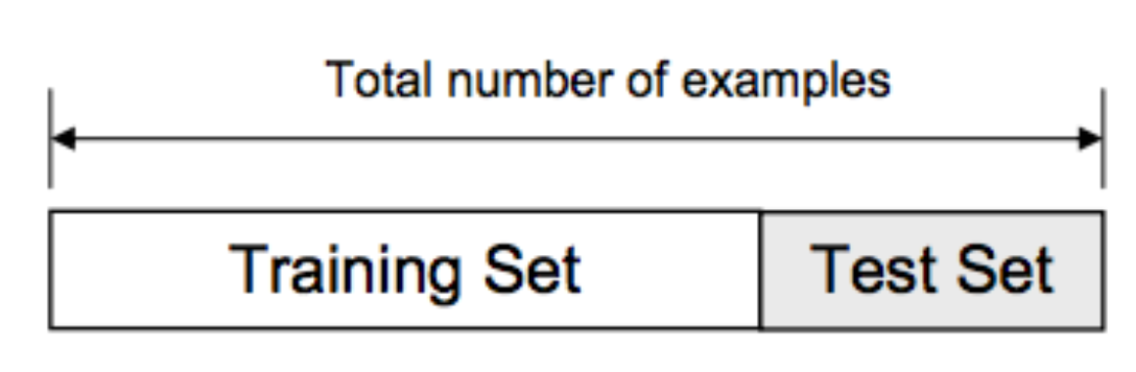
\includegraphics[width=10cm]{archivos/Datos/DataSplit}
                        \caption{https://towardsdatascience.com/train-test-split-and-cross-validation-in-python-80b61beca4b6. División de un conjunto de datos en datos de entrenamiento y test.}
                        \label{DataSplitImage}
                     \end{figure}


                \item Remuestreo


                    Estas técnicas permiten operar sobre el conjunto de datos para balancearlo, con el objetivo de que el modelo no se vea muy afectado debido a la diferencia de las clases mayoritarias respecto a las minoritarias. En este proyecto se han hecho uso de las siguientes técnicas de remuestreo:

                    
                    \begin{enumerate}

                        \item Downsampling: tiene como objetivo balancear el conjunto de datos para que todas las clases tengan el mismo número de muestras igualando el número de muestras de las clases mayoritarias a aquellas clases que contienen menos muestras, descartando aquellas que sobrepasen este límite. Aplicando esta técnica
                        \cite{Downsampling}

                        A LA ESPERA DE SABER SI ES LA MEJOR TECNICA

                        \item Generación de datos sintéticos: técnica que permite generar datos artificiales en base a los límites que separan unas clases de otras. Para la realización de este proyecto se ha hecho uso de la tećnica \glsentryfull{SMOTEII} \ref{SMOTEII}. Selecciona los vecinos más cercanos de la misma clase y genera nuevas muestras en base al espacio entre la clase minoritaria y sus vecinos más cercanos.\\

                        \glsentryshort{SMOTEII} ha sido utilizar para generar más muestras de los accidentes pertenecientes a las clases minoritarias (\textit{severos} y \textit{graves}).

                    \end{enumerate}

            \end{enumerate}



        \item Algoritmo Genético

            Para una correcto entrenamiento de un modelo predictivo es necesario optimizar los hiperparámetros con los que el modelo será entrenado. En este proyecto es necesario optmizar los hiperparámetros del algoritmo \glsentryshort{XGBoost}.\\

            Para ello se ha hecho uso de algoritmos genéticos \cite{GAXGBoostCode}, donde cada individuo perteneciente a la población de una generación está formado por una configuración de hiperparámetros específica, de tal forma que a lo largo de las iteraciones los individuos evolucionarán mediante el cruce y la mutación para dar lugar a nuevas configuraciones de hiperparámetros optimizadas \cite{GAXGBoostPaper}.

            Debido al coste computacional que tendría optimizar todos los parámetros debido al espacio de búsqueda y al no ser necesario tener en cuenta todos, se han seleccionado aquellos que más influencia tienen en el entrenamiento del modelo. Los hiperparámetros de los que consta cada individuo de la población son:

            \begin{enumerate}

                \item Profundidad máxima: es la máxima altura que puede tomar el árbol. Si el árbol de decisión alcanza demasiada profundidad tenderá al \textit{overfitting} ya que aprenderá relaciones complejas entre los datos que pueden deberse a ruido en los datos de entrenamiento.

                \item Peso mínimo de los hijos: es el mínimo peso que se establece a la hora de crear un nuevo nodo en el árbol. Cuando se entrena un árbol de decisión éste genera nuevos nodos en base a máxima separabilidad de los datos de entrenamiento en cada nivel. Con el límite de peso de los hijos establecemos un umbral mínimo de muestras que deben pertenecer a un nodo para realizar la separación. Un valor bajo en este parámetro permitirá crear nodos con menos muestras y por lo tanto el modelo tenderá al \textit{overfitting}.

                \item ETA: tamaño de paso utilizado para aplicar descenso por gradiente para minimizar la pérdida de los árboles anteriores.

            \end{enumerate}

            Una vez inicializados aleatoriamente los 100 individuos especificados en la población, 50 de ellos se seleccionarán y se cruzarán entre sí. Los parámetros de las nuevas soluciones mutarán dentro de unos límites específicos para cada parámetro establecidos como máximos y mínimos para que no se tomen valores extremos.

            En el proceso de evaluación, se entrenarán 100 modelos XGBoost instanciados con los valores de cada individuo en la población, de tal forma que la función \textit{fitness} será 

            SE HACE CON EL CONJUNTO DE ENTRENAMIENTO DOWNSAMPLED
            SE TESTA CON VALIDACION

            Para la 

        \item XGBoost

        \item Construcción de imágenes

            \cite{TASPCNN}

        \item Implementación de Modelos

            !!!!!!!!!!DE LA REVISION, CAMBIAR DE POSICION AQUI -> Función de activación CNN!!!!!!!!!!
            En el caso de este proyecto, se utilizará la función de activación \textit{Rectified Linear Unit (ReLU)} a la salida de cada capa de convolución, que se comporta devolviendo el valor $0$ para aquellas entradas que sean negativas y el valor original para aquellas que sean positivas, se puede apreciar el comportamiento en la figura \ref{RELUImage}.

            \begin{center}
                $f(x) = \left\{
                               \begin{array}{lr}
                                 0 & \text{if } x<=0\\
                                 x & \text{if } x>0
                               \end{array}
                        \right.$
            \end{center}

            \begin{figure}[h]
                \centering
                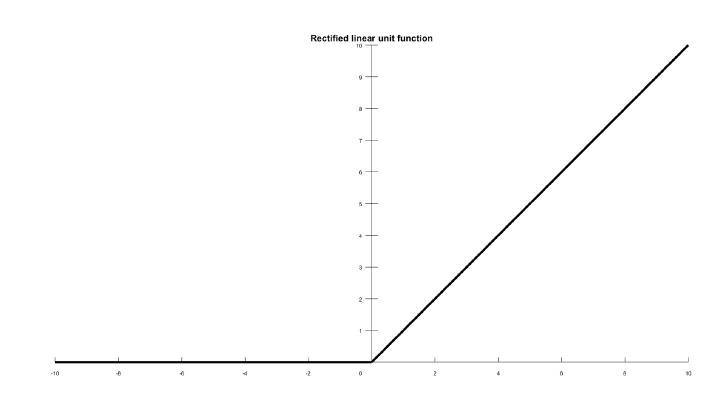
\includegraphics[width=10cm]{archivos/CNN/RELUImage}
                \caption{https://www.researchgate.net/journal/Transport-in-Porous-Media-1573-1634. Función ReLU}
                \label{RELUImage}
             \end{figure}
            !!!!!!!!!!FIN DE LA REVISION!!!!!!!!!!

            !!!!!!!!!!DE LA REVISION, CAMBIAR DE POSICION AQUI -> Función de activación CNN!!!!!!!!!!
            Una vez definidos los pasos que sigue el entrenamiento de una \textit{NN} y las características propias de las \textit{CNNs}, podemos hacer distinción entre los dos enfoques de \textit{CNNs} que se han aplicado en este proyecto. Cabe mencionar que el funcionamiento de ambas \textit{CNNs} únicamente difiere en el tamaño del \textit{kernel} y la forma en la que éste se desplaza debido a su dimensionalidad.
            !!!!!!!!!!FIN DE LA REVISION!!!!!!!!!!

            \cite{AutoSklearn}

    \end{enumerate}

\newpage
\section{Inserción de figuras}


Las figuras son un caso un poco especial ya que \LaTeX~busca el mejor lugar para ponerlas, no siendo necesariamente el lugar donde está la referencia. Por ello es importante añadirle un ``caption'' y un ``label'' para poder hacer referencia a ellas en el párrafo correspondiente. Nosotros ponemos la referencia a la figura \ref{multiimagen} que está en la página \pageref{multiimagen}, justo aquí debajo, pero \LaTeX ~puede que la ubique en otro lugar. (observa el código \LaTeX~ de este párrafo para observar como se realizan las referencias. Estos detalles también se aplican a tablas y otros objetos).



Existe también la posibilidad de realizarlo sin tablas, con subfiguras:
\begin{lstlisting}[style=Latex-color]
\begin{figure}[h]
    \centering
    \begin{subfigure}[b]{0.4\textwidth} % Espacio horizontal ocupado por la subfigura
    	\centering
        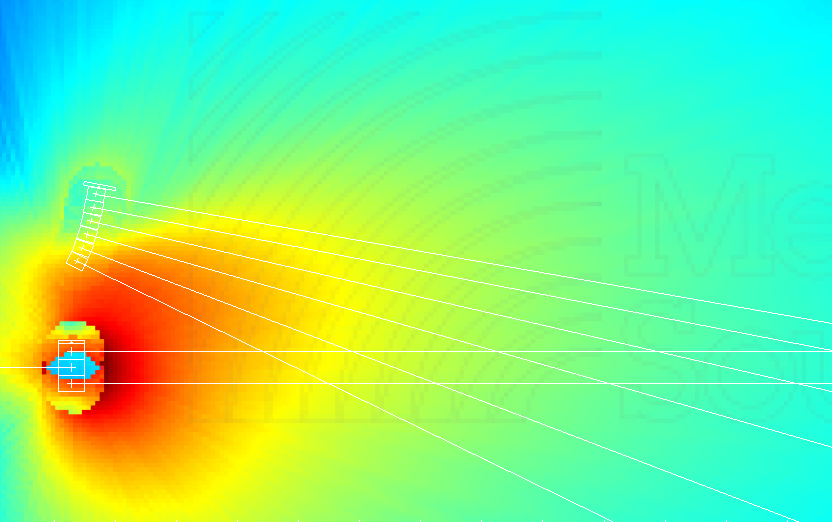
\includegraphics[width=4cm]{archivos/subs-sin} % Tamaño de la imagen
        \caption{Sin procesado.}
        \label{fig:gull}
    \end{subfigure}
    ~ % Añadir el espacio deseado, si se deja la linea en blanco la siguiente subfigura ira en una nueva linea
    \begin{subfigure}[b]{0.4\textwidth} % Espacio horizontal ocupado por la subfigura
    	\centering
        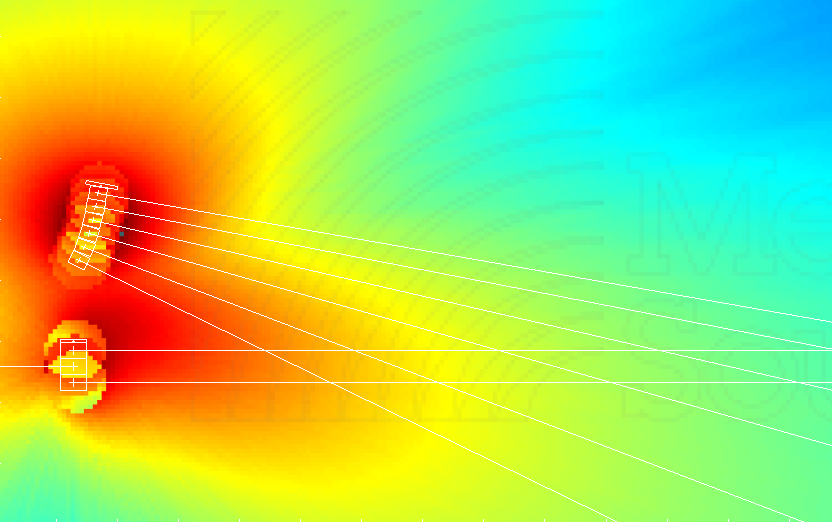
\includegraphics[width=4cm]{archivos/subs-con} % Tamaño de la imagen
        \caption{Con procesado.}
        \label{fig:tiger}
    \end{subfigure}
    \caption{Ejemplo de subfiguras}\label{sistemass}
\end{figure}
\end{lstlisting}
\begin{figure}[h]
    \centering
    \begin{subfigure}[b]{0.4\textwidth}
    	\centering
        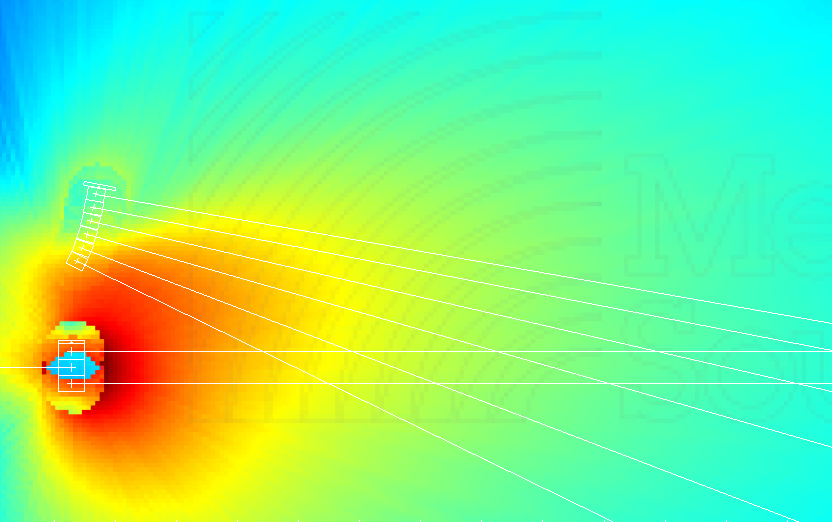
\includegraphics[width=4cm]{archivos/subs-sin}
        \caption{Sin procesado.}
        \label{fig:gull1}
    \end{subfigure}
    ~ % Añadir el espacio deseado, si se deja la linea en blanco la siguiente subfigura ira en una nueva linea
    \begin{subfigure}[b]{0.4\textwidth}
    	\centering
        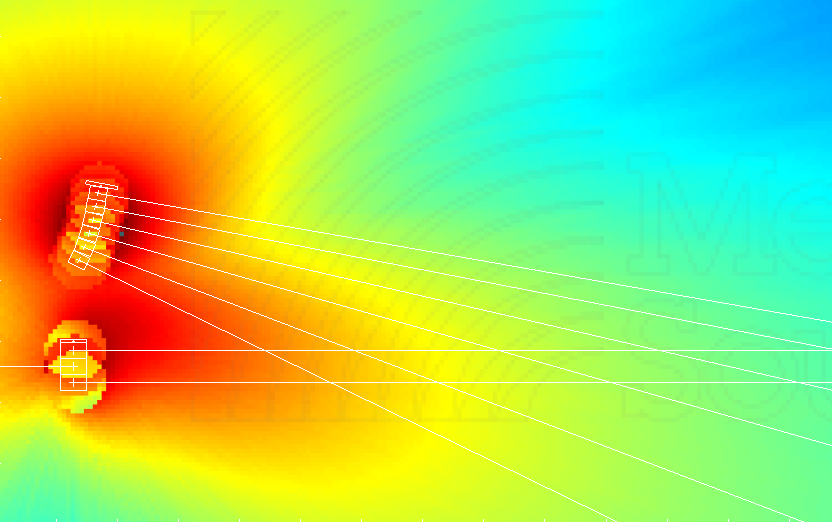
\includegraphics[width=4cm]{archivos/subs-con}
        \caption{Con procesado.}
        \label{fig:tiger1}
    \end{subfigure}
    \caption{Ejemplo de subfiguras}\label{sistemass1}
\end{figure}

\begin{figure}[h]
    \centering
    \begin{subfigure}[b]{\textwidth}
    	\centering
        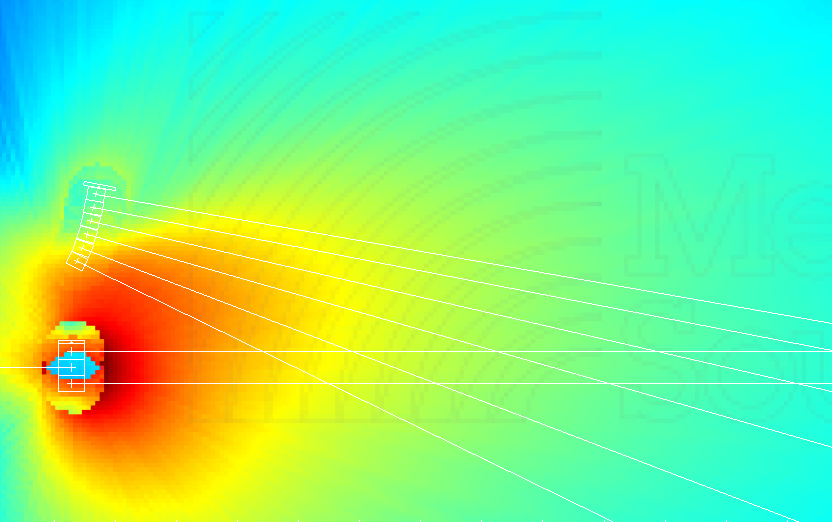
\includegraphics[width=4cm]{archivos/subs-sin}
        \caption{Sin procesado.}
        \label{fig:gull2}
    \end{subfigure}
    
    \begin{subfigure}[b]{\textwidth}
    	\centering
        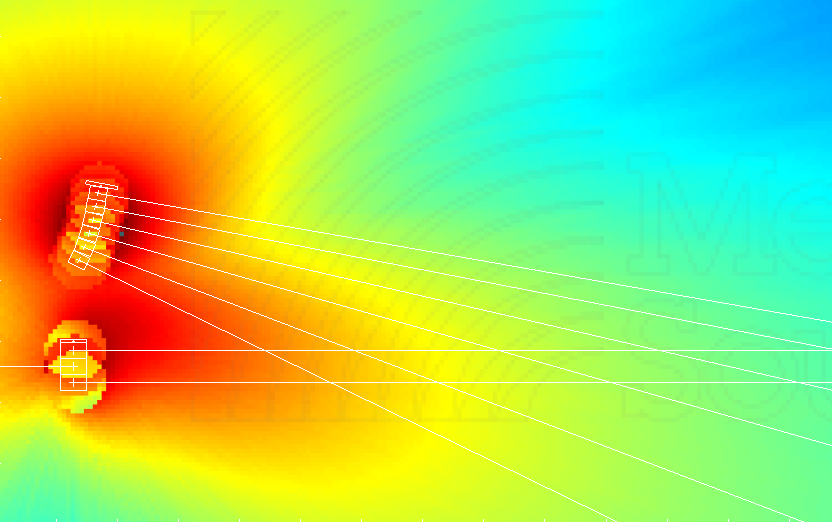
\includegraphics[width=4cm]{archivos/subs-con}
        \caption{Con procesado.}
        \label{fig:tiger2}
    \end{subfigure}
    \caption{Ejemplo de subfiguras vertical}\label{sistemass2}
\end{figure}

Si eliminas la línea '\textbackslash caption' de las subfiguras, tendrás las imágenes sin la información individual, aunque sí con la principal. Y obviamente, si eliminas el de la figura no se mostrará ninguna información.


\begin{table}[h]
\centering
\begin{tabular}{ccc}
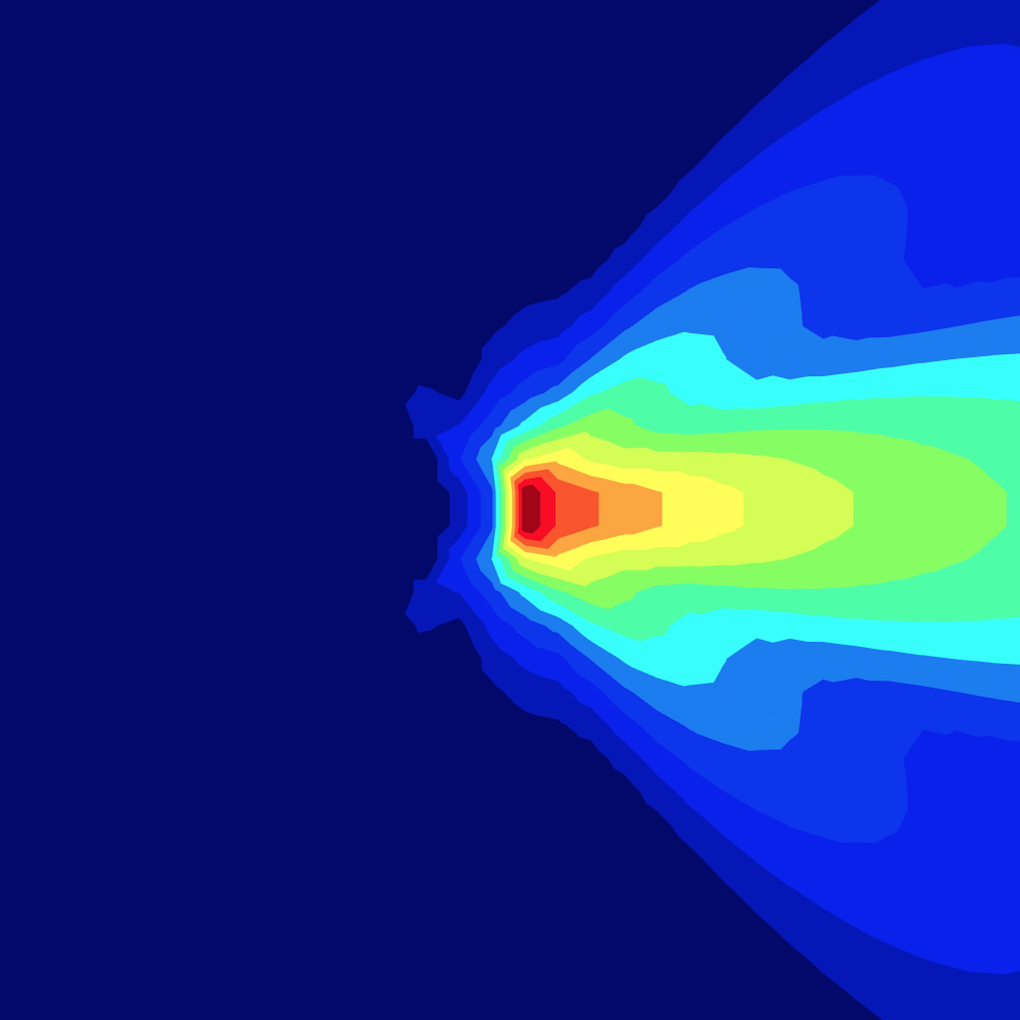
\includegraphics[scale=0.2]{archivos/130} & 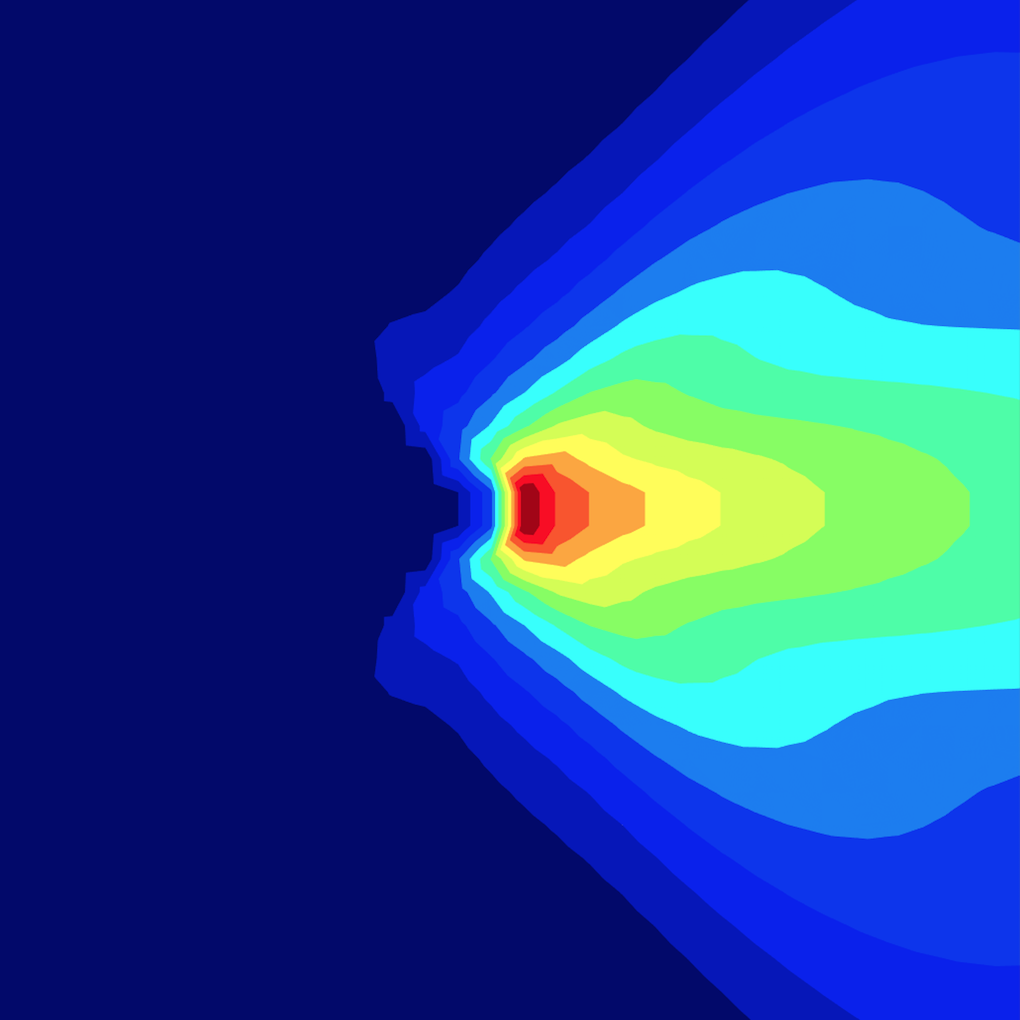
\includegraphics[scale=0.2]{archivos/160} & 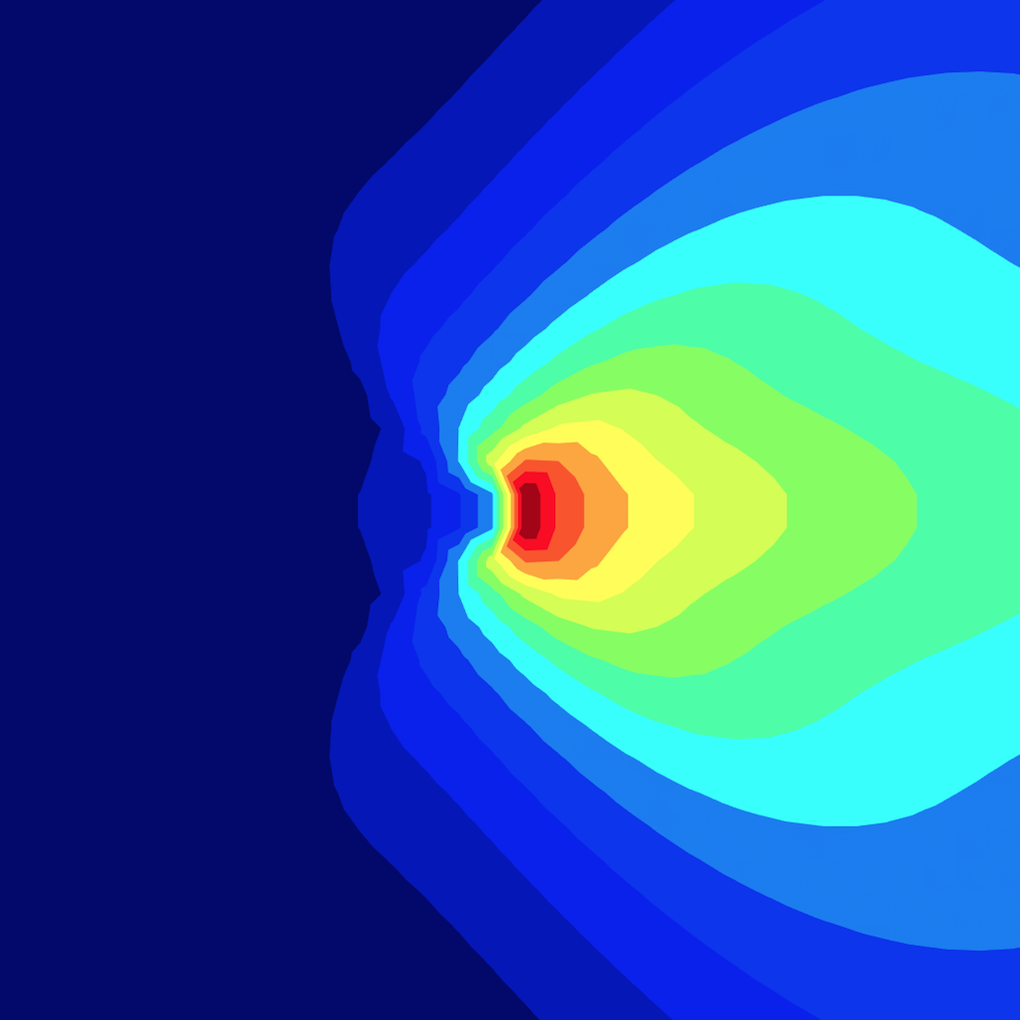
\includegraphics[scale=0.2]{archivos/190} \\
$Dist=1m \; ; \; \phi=30º$  & $Dist=1m \; ; \; \phi=60º$  & $Dist=1m \; ; \; \phi=90º$  \\
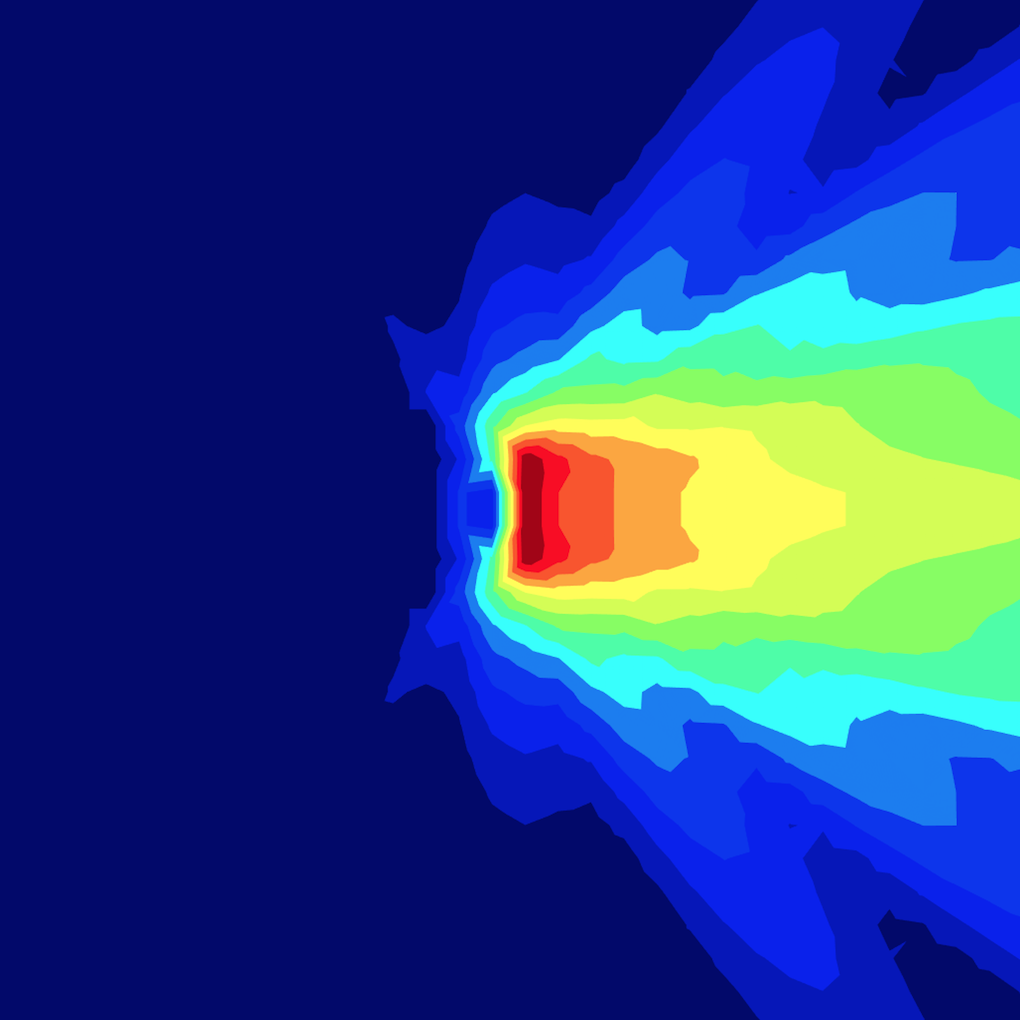
\includegraphics[scale=0.2]{archivos/230} & 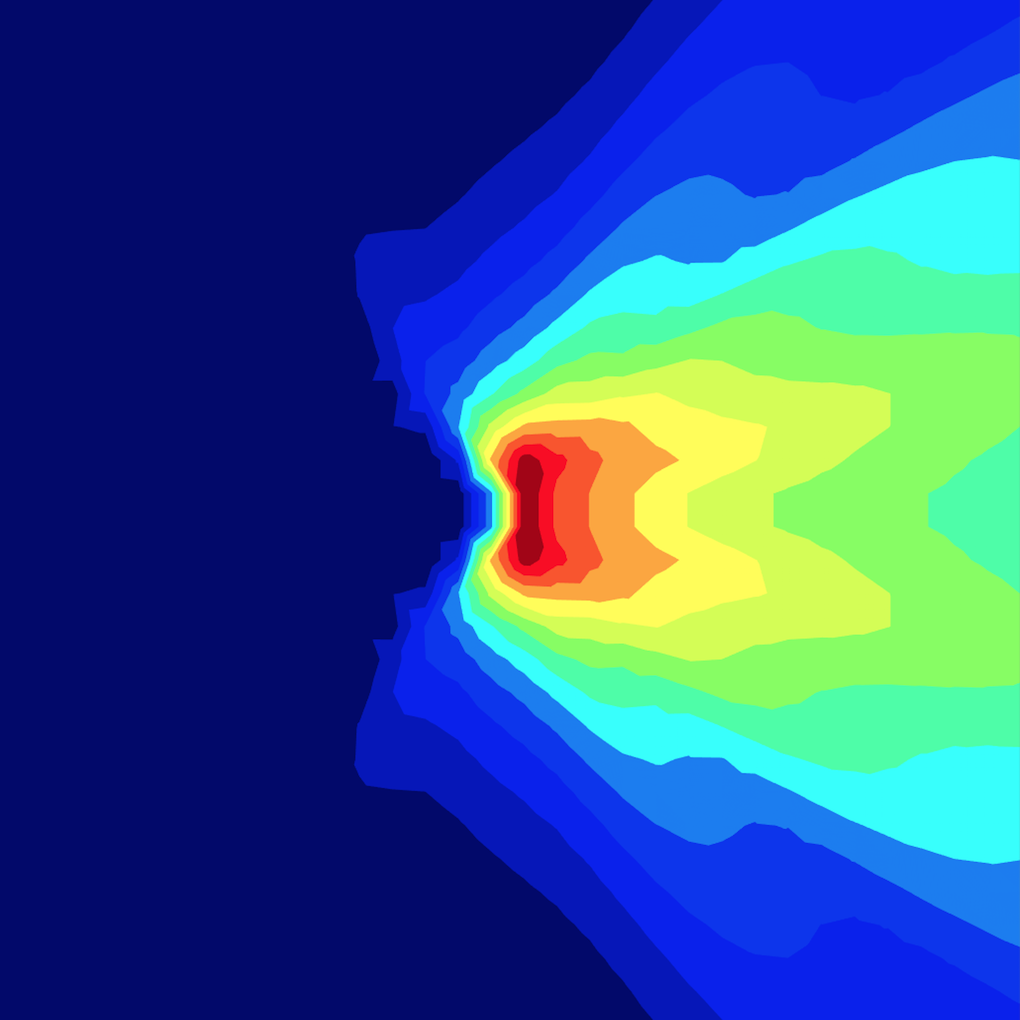
\includegraphics[scale=0.2]{archivos/260} & 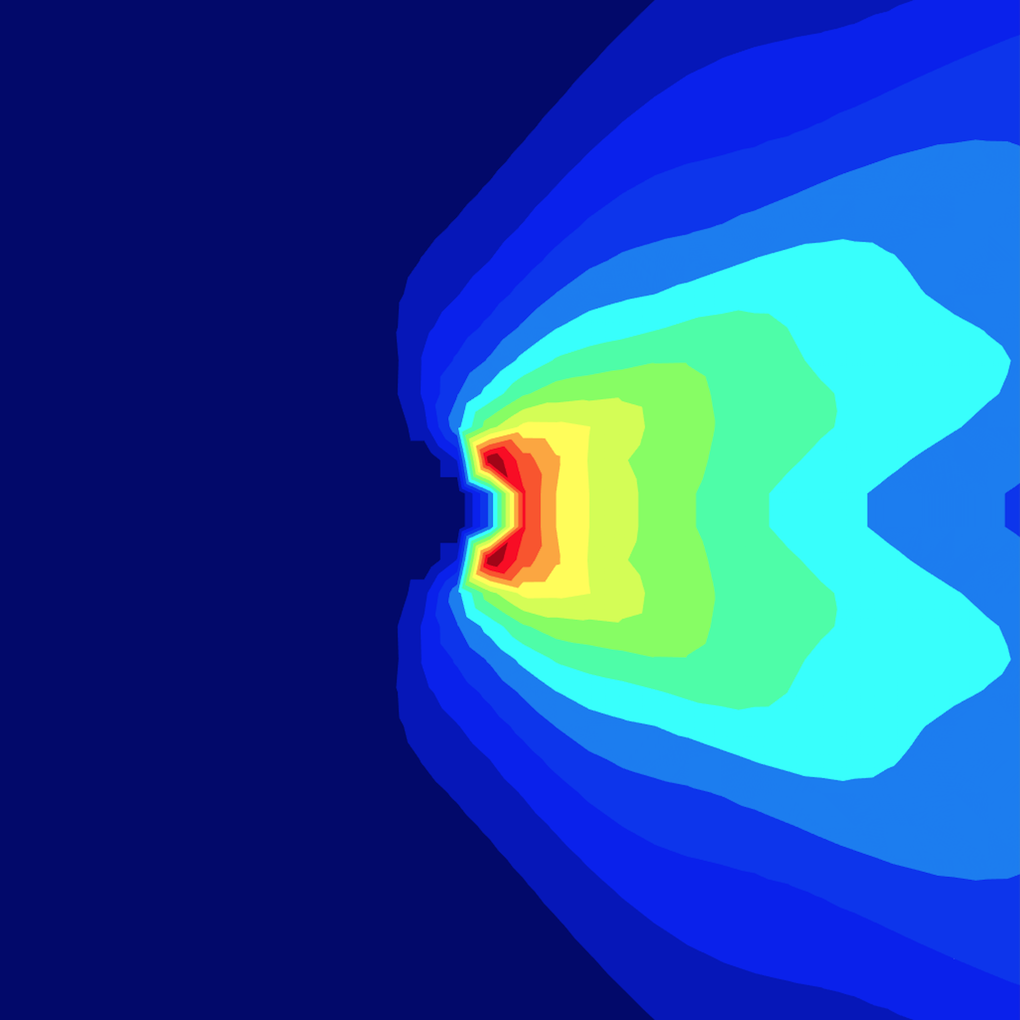
\includegraphics[scale=0.2]{archivos/290} \\
$Dist=2m \; ; \; \phi=30º$  & $Dist=2m \; ; \; \phi=60º$  & $Dist=2m \; ; \; \phi=90º$  \\
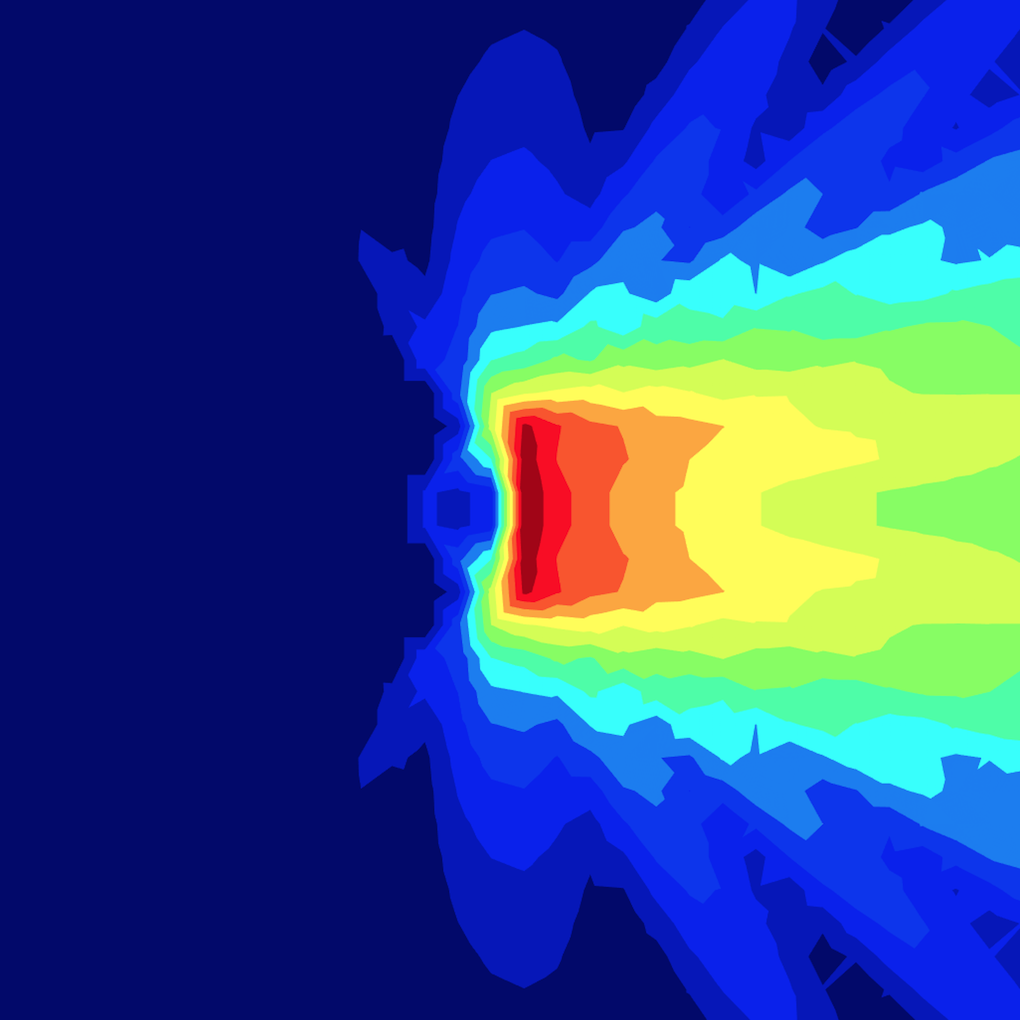
\includegraphics[scale=0.2]{archivos/330} & 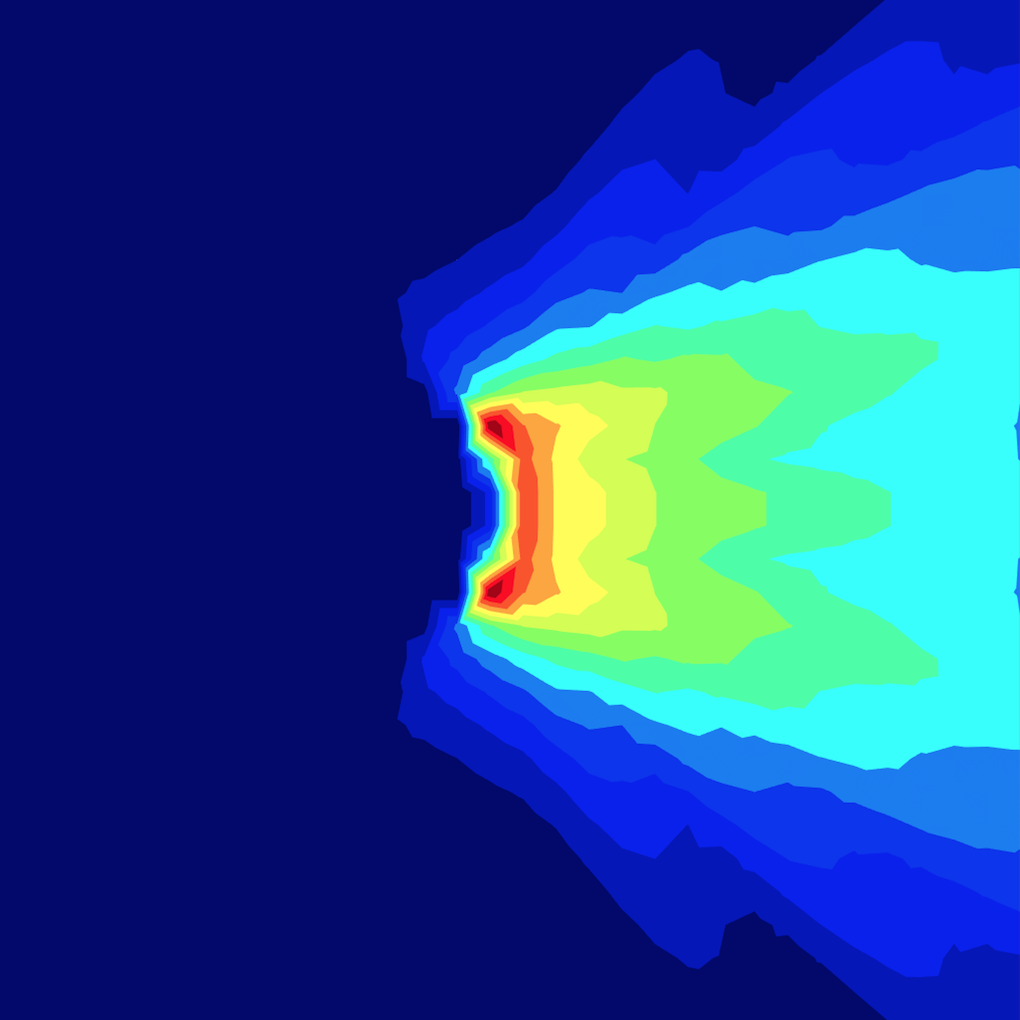
\includegraphics[scale=0.2]{archivos/360} & 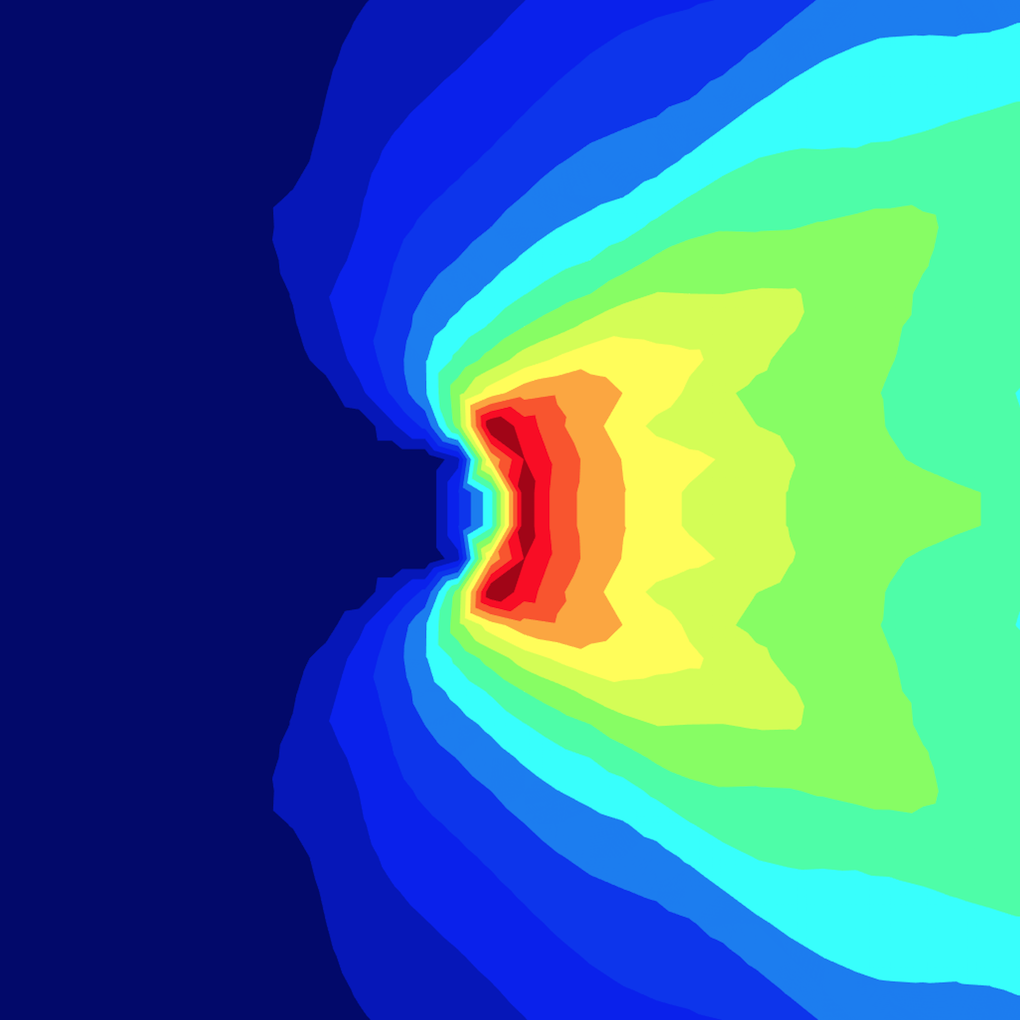
\includegraphics[scale=0.2]{archivos/390} \\
$Dist=3m \; ; \; \phi=30º$  & $Dist=3m \; ; \; \phi=60º$  & $Dist=3m \; ; \; \phi=90º$ \\
\end{tabular}
\caption{Esta es una tabla con múltiples imágenes. Útil cuando se deben mostrar varias juntas.}
\label{multiimagen} % 
\end{table}